\documentclass{beamer}
\mode<presentation>
\usetheme{CambridgeUS}
\usepackage[russian]{babel}
\usepackage[utf8]{inputenc}
\usepackage[T2A]{fontenc}
\usepackage{sansmathaccent}

\usepackage{verbatim}
\usepackage{alltt}

\pdfmapfile{+sansmathaccent.map}
\title[СУБД]{Нормализация отношений}
\author{Наумов Д.А., доц. каф. КТ}
\date[14.03.2020] {Базы данных и базы знаний, 2020}

\begin{document}

%ТИТУЛЬНЫЙ СЛАЙД
\begin{frame}
  \titlepage
\end{frame}
  
%СОДЕРЖАНИЕ ЛЕКЦИИ
\begin{frame}
  \frametitle{Содержание лекции}
  \tableofcontents  
\end{frame}
  
%РАЗДЕЛ 1
\section{Типы приложений: транзакционная и аналитическая обработка}
\begin{frame}
OLTP (On-Line Transaction Processing) — интерактивная транзакционная обработка.
\begin{itemize}
\item запросы пользователей выполняются одновременно - 
обработка идёт в режиме реального или приближенного к реальному времени;
\item запросы представляют собой интенсивный поток коротких операций по вставке, изменению и удалению небольшого числа записей в БД;
\item большая часть запросов известна на этапе проектирования;
\item время выполнения сложных аналитических запросов не является критическим для системы;
\end{itemize}
Примеры OLTP-приложений:
\begin{itemize}
\item системы складского учета;
\item системы заказа билетов;
\item банковские системы;
\end{itemize}
Данные OLTP-приложений \textbf{сильно нормализованы}.
\end{frame}

\begin{frame}
OLAP (On-Line Analytical Processing) - интерактивная аналитическая обработка. 
\begin{itemize}
\item Данные находятся \textbf{в режиме чтения}, за исключением моментов их обновления.
\item Выборки представляют собой \textbf{одиночные тяжёлые запросы}: поиски и расчёты по множеству \textbf{произвольных} критериев.
\item \textbf{Время отклика системы не регламентировано}.
\item Размеры базы данных на порядок и больше транзакционных.
\end{itemize}
\begin{block}{Пример типовой архитектуры OLAP}
\begin{center}
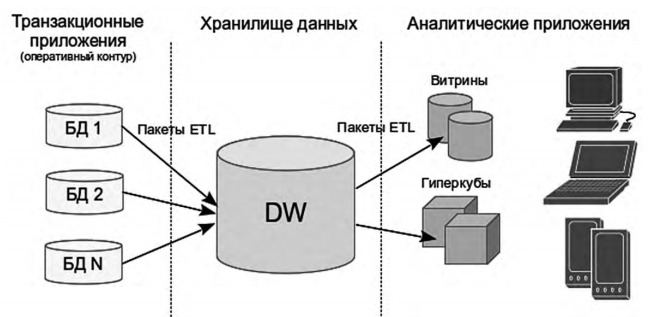
\includegraphics[scale=0.5]{images/olap.png}
\end{center}
\end{block}
\end{frame}

\section{Нормализация}
\begin{frame}
\begin{block}{Нормализация}
метод создания набора отношений с заданными свойствами на основе требований к данным, установленными в конкретной предметной области.
\end{block}
Цели нормализации:
\begin{itemize}
\item устранение избыточности при хранении данных, приводящей к увеличению размера БД.
\item исключение необходимости модификации данных в связных таблицах для минимизации времени и операций, проводящихся в одной транзакции.
\end{itemize}
Процесс нормализации:
\begin{enumerate}
\item исходная точка - представление предметной области в виде одного (или нескольких) отношений
\item на каждом шаге создается набор схем отношений, обладающих лучшими свойствами;
\item критерий <<лучше-хуже>> записит от целей проектирования.
\end{enumerate}
\end{frame}

\begin{frame}{Критерии оценки качества логичекой модели}
\begin{block}{Критерии оценки качества логичекой модели}
\begin{enumerate}
\item Адекватность базы данных предметной области.
\item Скорость выполнения операций обновления данных (вставка, обновление, удаление кортежей).
\item Скорость выполнения операций выборки данных.
\item Легкость разработки и сопровождения базы данных.
\item Отсутствие неоправданной избыточности данных.
\end{enumerate}
\end{block}
Критерии OLAP и OLTP:
\begin{itemize}
\item OLAP: на первый план выходит время отклика системы, данные могут быть избыточны.
\item OLTP: на первый план выходит обработка транзакций в режиме реального времени.
\end{itemize}
\end{frame}

\begin{frame}
\begin{block}{Избыточность данных}
одни и те же факты можно многократно получить из разных объектов базы данных
\end{block}
\begin{itemize}
\item польза: возможностm ускорения выполнения запросов;
\item избыточность должна быть контролируемой: необходима программная реализация проверок того, что избыточные и базовые данные адекватно согласованы между собой;
\end{itemize}
Расписание:
\begin{center}
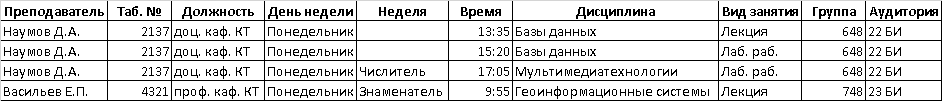
\includegraphics[scale=0.45]{images/ex-rasp-01.png}
\end{center}
Должности:
\begin{center}
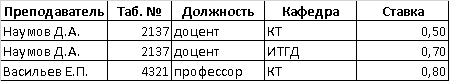
\includegraphics[scale=0.45]{images/ex-rasp-02.png}
\end{center}
\end{frame}

\begin{frame}
\begin{block}{Основные свойства нормальных форм}
\begin{itemize}
\item каждая следующая нормальная форма в некотором смысле улучшает свойства предыдущей;
\item при переходе к следующей нормальной форме свойства предыдущих нормальных форм сохраняются;
\end{itemize}
\end{block}
\begin{center}
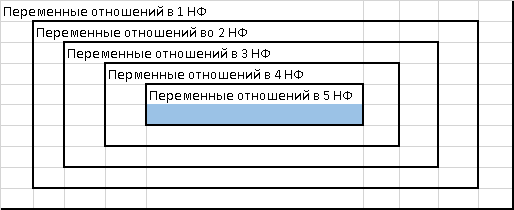
\includegraphics[scale=0.5]{images/forms.png}
\end{center}
\begin{block}{Схемы БД называются эквивалентными}
если содержание исходной БД может быть получено путем эквивалентного соединения отношений, входящих в результирующую схему, и при этом не появляется новых кортежей.
\end{block}
\end{frame} 

\begin{frame}
\begin{block}{1НФ - первая нормальная форма}
выполняется, если все значения атрибутов (колонок таблицы) атомарны, то есть неделимы.
\end{block}
\begin{itemize}
\item cобственные типы данных СУБД считаются атомарными, исключение
могут составлять массивы, в том числе символьные (текстовые) и байтовые.
\item атомарность может быть относительна выбранного взгляда со стороны предметной области и контекста. \end{itemize}
Пример 1: телефонный номер (в базе данных маркетинга, у телефонных операторов), колонки для хранения комментариев, целая и дробная части действительного числа, дата-время.

Пример 2: фамилия, имя, отчество в одной колонке.
\end{frame} 

\begin{frame}
\begin{block}{Пример}
\begin{center}
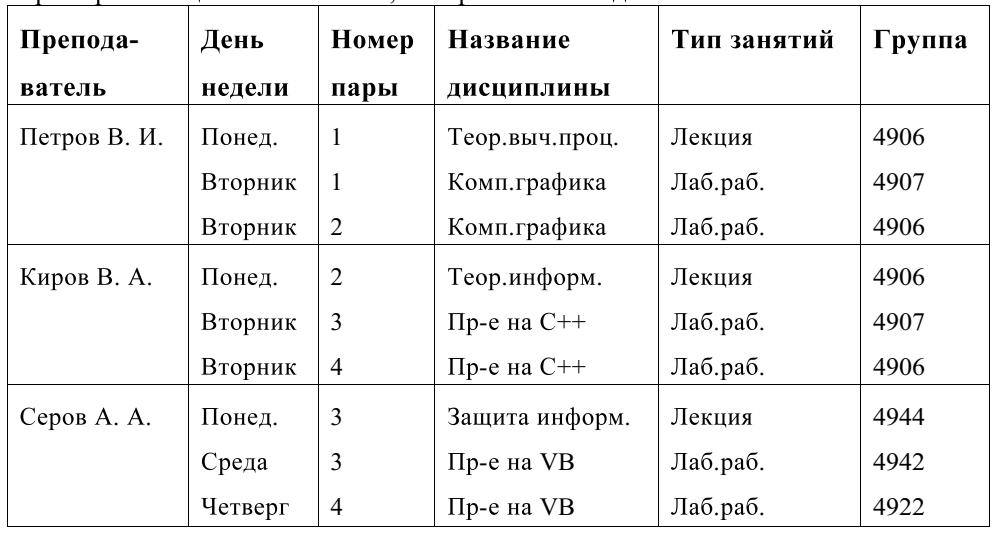
\includegraphics[scale=0.4]{images/nf-0.png}
\end{center}
\end{block}
\end{frame}

\begin{frame}
\begin{block}{Пример}
\begin{center}
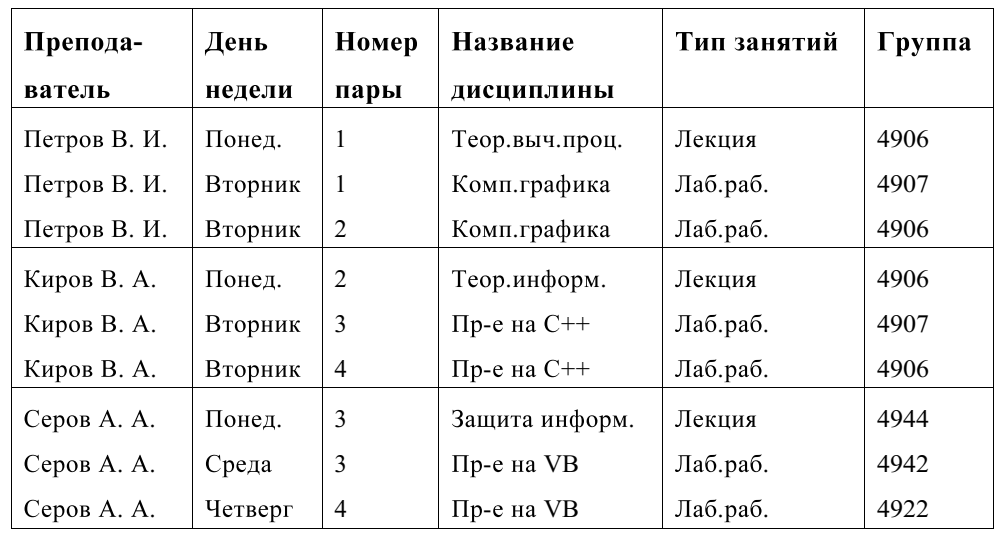
\includegraphics[scale=0.4]{images/nf-1.png}
\end{center}
\end{block}
\end{frame}

\begin{frame}
\begin{block}{2НФ - вторая нормальная форма}
означает, что выполнены требования 1НФ, при этом все атрибуты целиком зависят от составного ключа и не
зависят ни от какой его части.
\end{block}
\begin{itemize}
\item в определении говорится о ключах вообще, а не только о первичных. 
\item в отношении может быть несколько ключей, и некоторые из них могут являться составными
\end{itemize}
Пример 1: Описание продаж товара.

Пример 2: Сдача сессии (ФИО, №Зачетки, Группа, Дисциплина, Оценка).

Пример 3: Ключ - атрибут не выделенной еще сущности.
\end{frame}

\begin{frame}
\begin{block}{3НФ - вторая нормальная форма}
означает, что выполнены требования 2НФ, при этом в между атрибутами отношения нет транзитивных
зависимостей.
\end{block}
Пример: продажа каждой товарной позиции имеет своим основанием документ (заказ, счёт и т.д.), а её стоимость характеризуется ценой, количеством и валютой.

Транзитивные зависимости:
\begin{itemize}
\item Идентификатор продажи $\rightarrow$ Номер документа
\item Идентификатор продажи $\rightarrow$ Код валюты
\item Номер документа $\rightarrow$ Код валюты
\end{itemize}
Результатом нарушения 3НФ является избыточность хранения и необходимость обновления данных в связанной таблице.
\end{frame}

\begin{frame}
Пример: (ФИО, Номер зачетки, Группа, Факультет, Специальность, Выпускающая кафедра)
\begin{block}{Пример}
\begin{center}
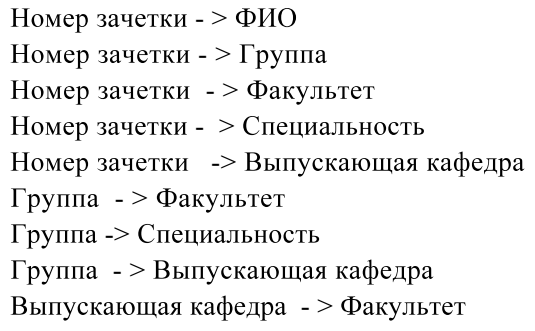
\includegraphics[scale=0.5]{images/nf-3.png}
\end{center}
\end{block}
\end{frame}

\begin{frame}
Допустимые схемы для OLAP: "снежинка", "звезда":
\begin{itemize}
\item центральным элементом являются таблицы фактов, содержащие события, транзакции, документы и др.
\item в таблице фактов одному документу (каждой его строке), соответствует одна запись.
\end{itemize}
\begin{block}{Денормализация документов в таблицу фактов}
\begin{center}
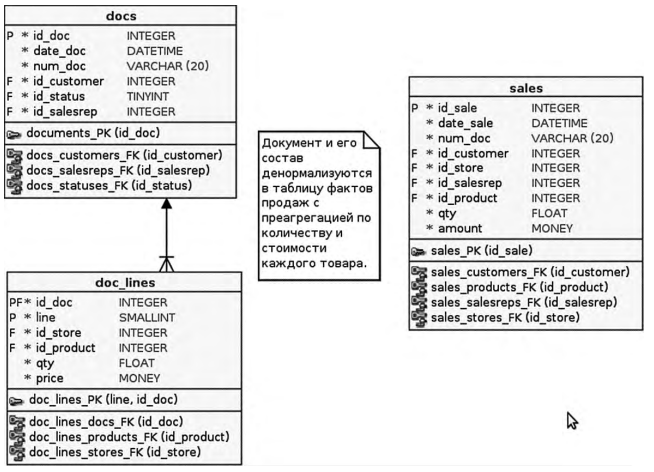
\includegraphics[scale=0.4]{images/denorm.png}
\end{center}
\end{block}
\end{frame}

\begin{frame}
\begin{block}{Пример SQL-запроса в транзакционной СУБД}
\begin{center}
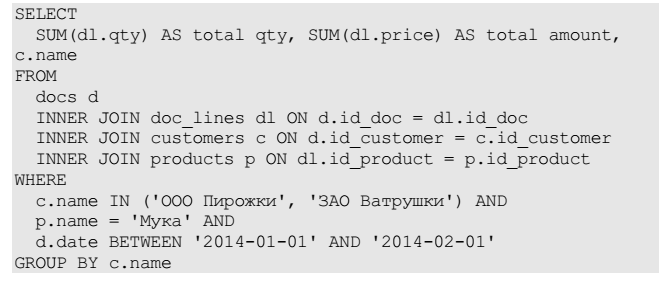
\includegraphics[scale=0.45]{images/sql-trans.png}
\end{center}
\end{block}
\begin{block}{Пример SQL-запроса в OLAP-СУБД}
\begin{center}
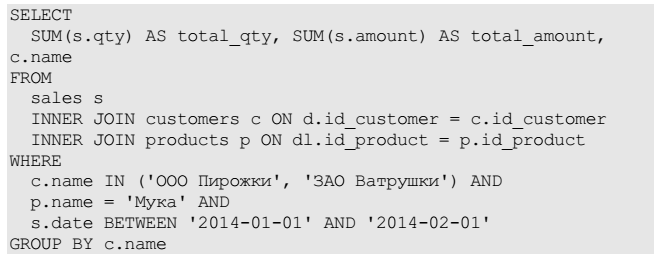
\includegraphics[scale=0.45]{images/sql-analitic.png}
\end{center}
\end{block}
\end{frame}

\begin{frame}
Если таблица фактов ссылается на таблицы-измерения, имеющие ссылки на другие измерения, то такая схема называется "снежинка".
\begin{block}{Таблица фактов в схеме "снежинка"}
\begin{center}
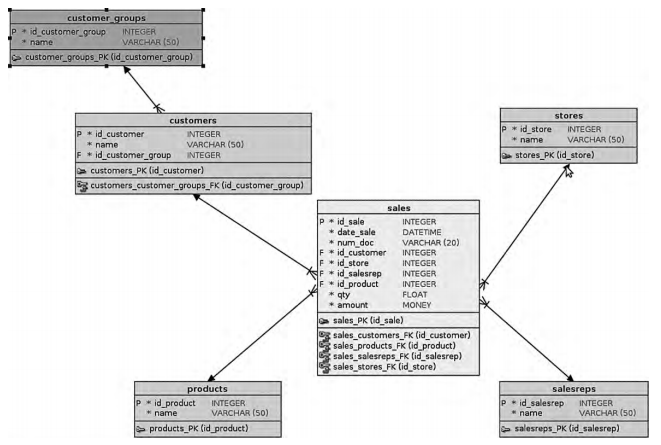
\includegraphics[scale=0.45]{images/snow.png}
\end{center}
\end{block}
Для запросов, включающих фильтрацию по группам клиентов, приходится делать дополнительное соединение.
\end{frame}

\begin{frame}
Схема "Звезда" полностью исключает иерархию измерений и необходимость соединения соответствующих таблиц в одном запросе.
\begin{block}{Таблица фактов в схеме "звезда"}
\begin{center}
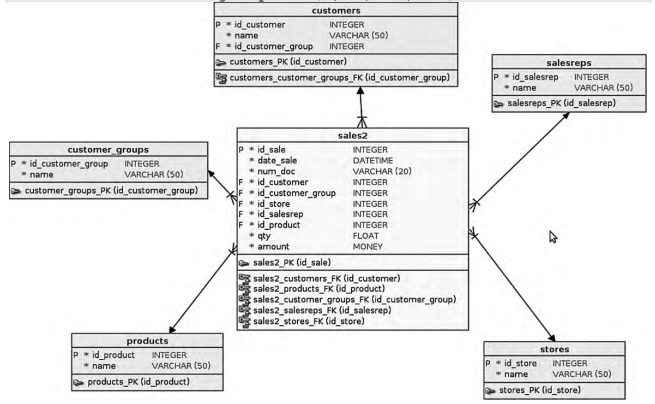
\includegraphics[scale=0.45]{images/star.png}
\end{center}
\end{block}
Обратной стороной денормализации всегда является избыточность, являющаяся причиной увеличения размера БД как в случае транзакционных, так и аналитических приложений.
\end{frame}


\begin{frame}
\begin{block}{Пример SQL-запроса в схеме "снежинка"}
\begin{center}
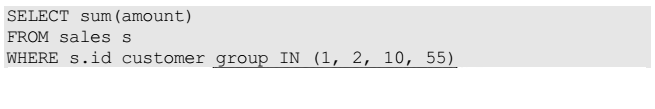
\includegraphics[scale=0.5]{images/star-sql.png}
\end{center}
\end{block}
\begin{block}{Пример SQL-запроса в схеме "звезда"}
\begin{center}
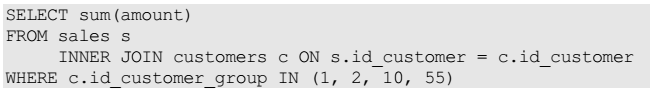
\includegraphics[scale=0.5]{images/snow-sql.png}
\end{center}
\end{block}
\begin{block}{Задача}
Посчитаем, примерную дельту на приведённом выше примере преобразования
"снежинки" в "звезду", если таблица продаж не использует компрессию данных и содержит
около 500 миллионов строк, а количество групп покупателей порядка 1000.
\end{block}
\end{frame}

\begin{frame}
\begin{itemize}
\item \textbf{теория нормализации является очень ценным достижением реляционной теории и практики}, поскольку она даёт научно строгие и обоснованные критерии качества проекта БД и формальные методы для усовершенствования этого качества;
\item идеи нормализации \textbf{полезны} для проектирования баз данных, они отнюдь н\textbf{е являются универсальным или исчерпывающим средством} повышения качества проекта БД - что существует слишком большое разнообразие возможных ошибок и недостатков в структуре БД, которые нормализацией не устраняются;
\item во всей сфере информационных технологий практически \textbf{отсутствуют методы оценки и улучшения проектных решений}, сопоставимые с \textbf{теорией нормализации реляционных баз данных} по уровню формальной строгости.
\end{itemize}
\end{frame} 

\end{document}